\chapter{Introduction and Preliminaries}
\label{chap:intro}

The exact treatment of strongly coupled and non Markovian open quantum
systems is a challenging problem.  If no analytical solution is
available, numerical methods have to be relied upon. Notably there are
HEOM\fixme{cite more}.

Besides the reduced dynamics of the system, the field of quantum
thermodynamics has attracted much interest. Quantum thermodynamics is,
among other issues, concerned with extending the standard
phenomenological thermodynamic notions to microscopic systems coupled
to macroscopic baths. This setting may make it possible to make
rigorous microscopic definitions of thermodynamic quantities such as
internal energy, heat and work that are consistent with the laws of
thermodynamics. There is no consensus on this matter yet, as is
demonstrated by the plethora of proposals and discussions in
\cite{Rivas2019Oct,Talkner2020Oct,Motz2018Nov,Wiedmann2020Mar,Senior2020Feb,Kato2015Aug,Kato2016Dec,Strasberg2021Aug,Talkner2016Aug,Bera2021Feb,Bera2021Jun,Esposito2015Dec}.

As system and baths may not be regarded as completely separable
entities in a strong coupling
regime~\cite{Rivas2019Oct,Esposito2015Dec}, an insight into the
dynamics of the bath is crucial. In some settings
\cite{Kato2016Dec,Lobejko2021Feb, Strasberg2021Aug}, such as cyclic
heat engines, the change in the bath energies is a quite suitable
definition of heat, as is expounded in
\cref{sec:basic_thermo,sec:operational_thermo}.

As it turns out, the framework of the ``Non Markovian State
Diffusion'' (NMQSD)~\cite{Diosi1998Mar}, which will be reviewed
in~\cref{sec:quick_hops}, allows access to certain bath related
observables such as the time derivative of the bath energy expectation
value and the interaction Hamiltonian expectation value. The

In \cref{sec:basic_thermo}, some operational quantum thermodynamical
questions will be discussed and some light will be shed on the
necessity of infinite baths.

\Cref{chap:flow} presents the main result of this thesis, namely
formulas to calculate expectation values of bath related
observables. Finally, we will discuss some numerical applications of
the result in \cref{chap:numres}. These application include a
\fixme{references}.

In \cref{chap:hops_notes}, some HOPS related subjects are discussed,
including a derivation of the HOPS for multiple baths embedded in an
auxiliary bosonic Fock space in \cref{sec:multihops}.

\newpage

\section{Open Systems, the NMQSD and HOPS}
\label{sec:quick_hops}

The basic and most general model which forms the foundation of all
matters discussed in this is a general quantum system \(H_\sys(t)\)
coupled to \(N\) baths of harmonic oscillators
\begin{equation}
  \label{eq:generalmodel}
  H(t) = H_\sys(t) + ∑_{n=1}^N \qty[L_n^†(t)B_n + \hc] + ∑_{n=1}^NH_B\nth ,
\end{equation}
with \(B_n=∑_{λ} g_λ\nth a_λ\nth\) and
\(H_B\nth=∑_λω_λ\nth \qty(a_λ\nth)^\dag a_λ\nth\). The \(a_λ\) are
bosonic annihilation operators and the \(L_n\) are arbitrary not
necessarily hermitian operators system Hilbert space. Sometimes
\cref{eq:generalmodel} is called the ``Standard Model of Open
Systems''. Throughout the work we set \(\hbar=c=1\).

Despite the simple structure of the baths, \cref{eq:generalmodel} is
generally very hard to solve beyond weak coupling strengths and the
secular approximation~\cite{Rivas2012}. The ``Non Markovian Quantum
State Diffusion'' (NMQSD)~\cite{Diosi1998Mar} approach allows to
recast \cref{eq:generalmodel} into a stochastic differential equation
in which the bath degrees of freedom are accounted for by Gaussian
stochastic processes. This drastic reduction of the number of degrees
of freedom also leads to an efficient numerical method, the
``Hierarchy of Pure States'' (HOPS).

The basics of the NMQSD will be briefly reviewed in
\cref{sec:nmqsd_basics} as will the basics of HOPS in
\cref{sec:hops_basics}. A more detailed account may be found in
\cref{sec:multihops} as well as \cite{RichardDiss}.

\subsection{Non Markovian Quantum State Diffusion}
\label{sec:nmqsd_basics}

We begin by considering a single zero temperature bath in the ground
state \(\ket{0}\). The total system-bath state may then be expanded in
a Bargmann coherent state basis~\cite{klauder1968fundamentals} with
respect to the bath degrees of freedom
\begin{equation}
  \label{eq:projected_single}
  \ket{ψ(t)} = ∫{\frac{\dd{\vb{z}}}{π^{N}}\eu^{-\abs{\vb{z}}^2}}\ket{ψ(t,\vb{z})^\ast}\ket{\vb{z}},
\end{equation}
where \(\vb{z}\) is a vector of coherent state labels \(z_λ\) for each
environment oscillator.

After transforming \cref{eq:generalmodel} into the interaction picture
with respect to \(H_B\) and using the properties of the coherent
states (\(\mel{z_λ}{a_λ}{ψ}\rightarrow ∂_{z_λ^\ast}\braket{z_λ}{ψ}\),
\(\mel{z_λ}{a_λ^\dag}{ψ}\rightarrow z_λ^\ast\braket{z_λ}{ψ}\)) we
arrive at
\begin{equation}
  \label{eq:nmqsd_single}
  ∂_tψ_t(η^\ast_t) = -\iu H ψ_t(η^\ast_t) +
  L {η}^\ast_tψ_t({η}^\ast_t) - L^†∫_0^t\dd{s}α(t-s)\fdv{ψ_t({η}^\ast_t)}{η^\ast_s},
\end{equation}
where \(α\) is the zero temperature bath correlation function (BCF)
\begin{equation}
  \label{eq:bcfdef}
  α(t-s) = \ev{B(t)B(s)} = ∑_λ \abs{g_λ}^2\,\eu^{-\iu ω_λ (t-s)}
\end{equation}
and \(η_t\) is a Gaussian stochastic process obeying
\begin{equation}
  \label{eq:single_processescorr}
  \begin{aligned}
      \mathcal{M}(η^\ast_t) &=0, & \mathcal{M}(η_tη_s) &= 0,
      & \mathcal{M}(η_tη_s^\ast) &= α(t-s).
  \end{aligned}
\end{equation}

Note that the BCF \(α\) is usually defined as Fourier transform of the
spectral density
\begin{equation}
  \label{eq:specdens}
  J(ω) = {π} ∑_λ \abs{g_λ}^2 δ(ω-ω_λ).
\end{equation}
One then usually performs a continuum limit so that \(J(ω)\) becomes
``smeared out'' to a smooth function and \(α(τ)\) decays to zero for
\(τ\rightarrow ∞\). This behavior leads to \cref{eq:nmqsd_single}



\subsection{Hierarchy of Pure States}
\label{sec:hops_basics}

\section{Ergotropy and Basic Thermodynamics of Open Systems}
\label{sec:basic_thermo}
The ergotropy of a quantum system is defined\fixme{mention paper that
  uses ergo for heat}
as~\cite{Binder2018}
\begin{equation}
  \label{eq:ergo_def}
  \ergo{ρ} = \max_{U\,\text{unitary}}\tr[\qty(ρ - UρU^\dag) H],
\end{equation}
which is the maximal energy that can be extracted from a system through
cyclic modulation of the Hamiltonian \(H\). A state is called passive
iff the maximizing \(U\) \cref{eq:ergo_def} is the identity \(\id\).

A passive state \(ρ_P\) is always diagonal in the eigenbasis of \(H\) and its
eigenvalues satisfy the following ordering condition~\cite{Lenard1978Dec}
\begin{equation}
  \label{eq:passive_diag}
  ρ_{p}=∑_{j=1}^{n} \lambda_{j}|j\rangle\langle j|, \quad E_{j} \leq E_{j+1}, \quad \lambda_{j+1} \leq \lambda_{j},
\end{equation}
where \(n<∞\) is the Hilbert space dimension. This condition is both
necessary and sufficient. Examples of passive states are the state of
the micro-canonical ensemble or a Gibbs state. Gibbs are further
distinguished by additional features as described
in~\cite{Lenard1978Dec}, which can be connected to formulations of the
zeroth and second laws of thermodynamics.

One of these properties is complete passivity. Completely passive
states remain passive under the transformation \(ρ\to\otimes^Nρ\) (and
an \(N\)-fold sum of the Hamiltonian) for finite \(N\). Therefore no
energy can be extracted from multiple identical systems at the same
temperature. For finite dimensional systems, the complete passivity
implies the form of the Gibbs state. The open-systems case differs as
here a ``small'' system is coupled to a bath of infinite size. If the
system state is not a Gibbs state, the whole system becomes
non-passive, even if the system state is passive with respect to the
system Hamiltonian\footnote{for example being the ground state}.

For systems of infinite size, states fulfilling the
Kubo–Martin–Schwinger (KMS) condition have been proposed as the
generalizations of Gibbs states, having similar properties as
Gibbs states. Under some conditions passivity implies the KMS
condition. These conditions are related to the fact that KMS states
are not necessarily unique~\cite{Binder2018,Pusz1978Oct}.

The KMS condition is stated for two arbitrary observables \(A,B\) and
\(F_{AB}(t)=\tr[ρ_βA(t)B(0)]\) (Heisenberg picture,
\(A(t)=\eu^{\iu H t}H\eu^{-\iu H t}\)) as
\begin{equation}
  \label{eq:kmscond}
  F_{AB}(-t) = F_{BA}(t-\iu β)
\end{equation}
by virtue of analytic continuation.

For two initially uncorrelated KMS states, of different
temperature, the Carnot efficiency bound can be
proven~\cite{Pusz1978Oct}.

A simple application of ergotropy is an explanation for quantum
friction. The buildup of coherence\footnote{Meaning a state which is
  non-diagonal in the energy basis.} in a quantum system makes the
state non-passive and thus requires additional energy which cannot be
extracted by modulating of the energy level gaps of the
system\footnote{This is the usual mechanism of energy extraction in a
  quantum Otto cycle~\cite{Geva1992Feb}.}~\cite{Kurizki2021Dec}.  The
reduction of efficiency in through quantum coherence general has been
termed quantum friction. However, the occurrence of coherence does not
have to lead to a reduction in efficiency\fixme{do more research on
  that.refer to simulations}, if a diagonal state is restored \footnote{Shortcuts to
  adiabaticity, see for example~\cite{Chen2010Feb}.}.

\subsection{The Ergotropy of Finite Systems Coupled to a Thermal Bath}
\label{sec:ergoonebath}

Let us consider models with the Hamiltonians
\begin{equation}
  \label{eq:simple_bath_models}
  H = \id_\sys\otimes H_\bath + H_\sys\otimes \id_\bath,
\end{equation}
where the system \(\sys\) is finite dimensional and \(H_\bath\) may
chosen arbitrarily. Let the initial state of the system be
\begin{equation}
  \label{eq:simple_initial_state}
  ρ=ρ_\sys\otimes τ_β,
\end{equation}
where \(τ_β=\eu^{-β H_\bath}/Z\) and \(ρ_\sys\) is arbitrary.

An interesting question is whether the ergotropy of such a state is
finite. This amounts to the formulation of the second law: ``No energy
may be extracted from a single bath in a cyclical manner''.
For systems obeying GKSL dynamics connected to a KMS state heat bath,
thermodynamic laws can be derived in certain situations\footnote{very
  slow or very fast modulation of the system
  hamiltonian}\cite{Binder2018}, which imply the answer ``yes'' for the
above questions. In the non-Markovian case, those arguments do not
hold anymore.

For finite dimensional baths, we always have finite ergotropies, as
their Hamiltonians are bounded. In the infinite dimensional case, we
may expect that the ergotropy is still finite for some models, as long
as the energies of the thermal states for those models is finite. This
assumption breaks down when we consider infinite baths, whose thermal
energy is unbounded even for finite temperatures.

Nevertheless, \fixme{graphics} the ergotropy appears to be
bounded. Further, the system as if it was in a passive state as soon
as the limit cycle is reached. In fact, there is a simple and general
argument that provides and upper bound on the ergotropy of states of
the form~\cref{eq:simple_initial_state} based on the special form of
Gibbs states and relative entropy. The latter quantity allows the
application of quantum informational tools, even in the presence of
infinite baths if we are careful in taking limits.

The following is adapted
from~\cite{Biswas2022May,Alicki2013Apr,Lobejko2021Feb} and we limit
ourselves to finite dimensional problems for now.  As unitary
transformations leave the entropy invariant
(\(\tr[ρ\ln(ρ)] = \tr[ρ_P\ln(ρ_P)]\)), we have for an arbitrary
\(β > 0\) and \(ρ_β=\exp(-βH)/Z\)
\begin{align}
    \ergo{ρ} &= E(ρ) - E(ρ_P) = \tr[(ρ-ρ_P) H]\nonumber\\
             &= -\frac{1}{β}\tr[(ρ-ρ_P)
               \qty(\ln(ρ_β) + \ln(Z))] \nonumber\\
             &= -\frac{1}{β}\tr[(ρ-ρ_P) \ln(ρ_β)] =
               -\frac{1}{β}\tr[(ρ-ρ_P) \qty(\ln(ρ_β))]\nonumber\\
             &=\frac{1}{β}\qty[\tr[ρ(\ln(ρ) - \ln(ρ_β))] -
               \tr[ρ_P(\ln(ρ_p) - \ln(ρ_β))]]\nonumber\\
             &\equiv\frac{1}{β}\qty[\qrelent{ρ}{ρ_β} - \qrelent{ρ_P}{ρ_β}]\label{eq:ergo_entro},
\end{align}
where we have used \(\tr[ρ]=\tr[ρ_P]=1\).

The relative entropies
appearing in \cref{eq:ergo_entro} are always finite, as \(ρ\) is
finite-dimensional and \(ρ_β\) has full rank.  As energy is minimized
by a Gibbs state when keeping the entropy fixed, we find an upper
bound on the ergotropy by replacing \(ρ_P\to ρ_{β^\ast}\) in
\cref{eq:ergo_entro} where
\(S(ρ_{β^\ast})=S(ρ)\)~\cite{Alicki2013Apr}.

By choosing the temperature in \cref{eq:ergo_entro} accordingly, we
arrive at
\begin{equation}
  \label{eq:ergo_bound_single}
  \ergo{ρ} \leq \frac{1}{β^\ast}\qrelent{ρ}{ρ_{β^\ast}}.
\end{equation}
This bound can be saturated for states which are a permutation of a
thermal state, as their corresponding passive states is the thermal
state.

For our setting in
\cref{eq:simple_bath_models,eq:simple_initial_state} we find a still
better way to bound the ergotropy and fix the
temperature~\cite{Lobejko2021Feb}. Substituting \(ρ\to ρ \otimes τ_β\)
in \cref{eq:ergo_entro} we obtain
\begin{equation}
  \label{eq:thermo_ergo_bound}
  \begin{aligned}
  \ergo{ρ\otimes τ_β} &= \frac{1}{β}
  \qty[\qrelent{ρ\otimes τ_β}{ρ_β\otimes τ_β} - \qrelent{(ρ\otimes
                        τ_β)_P}{ρ_β\otimes τ_β}]\\
    &=\frac{1}{β}
  \qty[\qrelent{ρ}{ρ_β} - \qrelent{(ρ\otimes τ_β)_P}{ρ_β\otimes
      τ_β}] \leq \frac{1}{β} \qrelent{ρ}{ρ_β}.
  \end{aligned}
\end{equation}

Remarkably, the bound \cref{eq:thermo_ergo_bound} only depends on the
system state and ``inherits'' the temperature of the bath. For any
\(\dim[τ_β] = N\gg 1\) the bound stays valid. It is therefore
reasonable to expected that it is also valid for an infinite bath. On
the basis of physical intuition, a very large but finitely sized bath
may be an arbitrarily good substitute for a continuous one. One might
even argue, that the continuous bath is a mathematically convenient
construct and the finite bath is the physical one.  The objection to
taking the limit outright is that the state \(τ_β\) does not exist as
trace class operator for an infinite bath.

Interestingly, a saturation of \cref{eq:thermo_ergo_bound} is achieved
in~\cite{Skrzypczyk2014Jun} with a continuous qubit
bath. In~\cite{Lobejko2021Feb} a more generic argument is made in a
similar setting. Both propose concrete protocols within the bounds of
thermal operations and by considering explicit work reservoirs.

For the term \(\qrelent{(ρ\otimes τ_β)_P}{ρ_β\otimes τ_β}\) to vanish
in \cref{eq:thermo_ergo_bound}, the state bath and system should be as
close to the product thermal state as possible and so the bath state
should not change too much. This is achievable with a continuous
infinite size bath.  As \(ρ_β\otimes τ_β\) is the steady state of GKSL
dynamics (without modulation) under mild
assumptions~\cite{Binder2018}, it can be said that in this case
ergotropy is being lost.

A corollary of \cref{eq:thermo_ergo_bound} is the Clausius form of the
second law. By setting the system Hamiltonian to \(α \id\) in the
above discussion the ergotropy becomes the change of bath energy
\begin{equation}
  \label{eq:ergo_bath_change}
  \begin{aligned}
    \ergo{ρ} &= \max_{U\,\text{unitary}}\tr[\qty(ρ - UρU^\dag)
               (α\id\otimes H_\bath)] \\
             &=\max_{U\,\text{unitary}}\tr_\bath[\qty(\tr_\sys[ρ-UρU^\dag])
               H_\bath]\\
             &\equiv\max_{U\,\text{unitary}}ΔE_\bath\leq \frac{1}{β}\qrelent{ρ}{\frac{\id_N}{N}},
  \end{aligned}
\end{equation}
where \(N\) is the system dimension. No finite amount of energy may
therefore be extracted from the bath in a periodic manner. If it were
possible to extract a constant positive amount of energy from the bath
per cycle, \cref{eq:ergo_bath_change} would be breached in finite
time.


\subsection{Notes on the Ergotropy of a Bath of Identical Oscillators
  and a Two Level System}
\label{sec:explicitergo}
Here, we explicitly calculate the ergotropy of a finite dimensional
system connected to a bath of identical oscillators. Throughout we
will set the zero-point energy of the oscillators to zero, meaning
that \(H=ωa^\dag a\) for a single harmonic oscillator with the usual
annihilation operator \(a\).


Let us choose \(H_S=α\id_N\)  for simplicity,
where \(α\) is an arbitrary energy scale. The ergotropy is then equal
to the maximal energy reduction of the bath under arbitrary cyclic
modulation.

The bound \cref{eq:thermo_ergo_bound} further simplifies to
\begin{equation}
  \label{eq:thermo_ergo_bound_specific}
  \ergo{ρ\otimes τ_β} \leq \frac{1}{β} \qty[\ln(N) - S(ρ)],
\end{equation}
where \(S(ρ)=-\tr[ρ\ln(ρ)]\).  For a pure state
\cref{eq:thermo_ergo_bound_specific} is maximal and we therefore choose
\(ρ=\ketbra{0}\) as an arbitrary pure state.

If we take the system to be a qubit, the right hand side of
\cref{eq:thermo_ergo_bound_specific} is the Landauer bound
\(β^{-1}\ln2\). Therefore, up saturation of the bound
\cref{eq:thermo_ergo_bound_specific} we can extract enough energy from
the bath to erase one bit in a system of the same temperature as the
bath. Indeed, owing to \cref{eq:thermo_ergo_bound_specific} the closer
the qubit state is to the infinite temperature (erased) state the more
certain we are, that we have extracted the maximum energy out of the
bath.


\paragraph{One Oscillator}
As a demonstration of the general program, let us first discuss the
ergotropy of a single harmonic oscillator with frequency \(ω\) as a
bath.  The initial state is given by
\begin{equation}
  \label{eq:onehoinit}
  ρ_{0} = ∑_{n=0}^{∞} \underbrace{Z^{-1}\eu^{-βωn}}_{λ_{0,n}} \ketbra{{0,n}},
\end{equation}
where \(Z=Z_{1}=\frac{1}{1-\eu^{-βω}}\) is the partition sum of one
bosonic mode with frequency \(ω\).

In contrast to the state characterized by \cref{eq:passive_diag} we
only fill every second level with \cref{eq:onehoinit}. To construct a
corresponding passive state\footnote{Due to the degeneracy of the
  system Hamiltonian, the passive state is not unique.} we have to
construct a sequence \(λ_{i},\, i \in \NN_{0}\) out of the weights
\(λ_{0,n}\) such that \(λ_{i}\geq λ_{j}\) for \(i\leq j\) and a
sequence of states \(\ket{j}\) so that for \(\ev{H}{j} = E_{j}\) we
have \(E_{i}\leq E_{j}\) for \(i\leq j\). The passive state and its
corresponding energy is then
\begin{equation}
  \label{eq:specific_passive_state}
  \begin{aligned}
    ρ_{p} &= ∑_{i} λ_{i} \dyad{i} & E_{p} &= ∑_{i} λ_{i}E_{i}.
  \end{aligned}
\end{equation}

In the present case, this is easily done by defining \(λ_{i}=λ_{0,i}\)
and
\begin{equation}
  \label{eq:state_enumeration_single}
  \ket{i} =
  \begin{cases}
    \ket{0, i/2} & i\text{ even} \\
    \ket{1, (i - 1) / 2} & i\text{ odd}. \\
  \end{cases}
\end{equation}

Thus, we find a passive state
\begin{equation}
  \label{eq:one_ho_pass}
  ρ_{p} = \frac{1}{Z} \qty[∑_{i} \eu^{-2i βω} \ketbra{0, i} +
  \eu^{-(2i + 1) βω} \ketbra{1, i}].
\end{equation}

The corresponding energy difference \(\ev{H (ρ_{0} - ρ_{p})}\) works
out to be
\begin{equation}
  \label{eq:one_ho_ergo}
  \mathcal{W} = ω\qty(\frac{1}{\eu^{βω} - 1} - \frac{1}{\eu^{2βω} - 1}) = ω \frac{\eu^{-β ω} - \eu^{-2 β ω}}{1-\eu^{-β
      ω}-\eu^{-2 β ω} + \eu^{-3 β ω}} \xrightarrow{βω
    \rightarrow ∞} \frac{ω}{\eu^{βω} - 1}.
\end{equation}

For low temperatures or large frequencies, the ergotropy of the
oscillator is just its mean thermal energy \(ω\bose(ωβ)\). In the
opposite limit we find
\(\mathcal{W} = \frac{1}{7β}< β^{-1}\ln(2)\)\fixme{check calculations
  :P}.

\paragraph{Many Oscillators}
For the case of \(N>1\) oscillators with frequency \(ω\) the initial
state is
\begin{equation}
  \label{eq:manyhoinit}
  ρ_{0} = ∑_{\vb{n}\in\ZZ_{0}^{n}} \underbrace{Z^{-1}\eu^{-βω\abs{\vb{n}}}}_{λ_{0,\vb{n}}} \ketbra{{0,\vb{n}}},
\end{equation}
with the \(n_{i}=(\vb{n})_{i}\) labeling the state of the \(i\)th
oscillator and \(\abs{\vb{n}}=∑_{i=1}^{N}n_{i}\) and \(Z=Z_{1}^{N}\).

In this case we again call the ordered sequence of weights \(λ_{i}\),
but its construction is somewhat more complicated and we will refrain
from doing so here explicitly.
Instead we take an enumeration of state labels
\(\{\vb{n}^{i}\}_{i\in\NN_{0}}\) such that
\(i<j \implies m_{i} \leq m_{j}\) with
\(m_{i}\equiv\abs{\vb{n}^{i}}\). The energies of the states
\(\ket{k,\vb{n}^{i}}\) evaluate to \(E_{k, i} = ω m_{i}\) and the
weights to \(λ_{0,i}=Z^{-1}\eu^{-βω m_{i}},\,λ_{1,i}=0\).

The required enumeration of states and energies is then
\begin{equation}
  \label{eq:many_enum}
  \begin{aligned}
  \ket{i} &=
  \begin{cases}
    \ket{0, m_{i/2}} & i\text{ even} \\
    \ket{1, m_{(i-1)/2}} & i\text{ odd}
  \end{cases},
    & E_{i} &= ω m_{\lfloor{i/2}\rfloor}
  \end{aligned}
\end{equation}
and the enumeration of weights is \(λ_{i} = λ_{0,i} =Z^{-1}\eu^{-βω m_{i}}\).


The corresponding passive state energy will be
\begin{equation}
  \label{eq:many_ho_pass}
  E_{p} = \frac{ω}{Z} ∑_{i=0}^{∞} m_{i} \pqty{\eu^{-ωβ m_{2i}} + \eu^{-ωβ m_{2i+1}}}.
\end{equation}

For each value of \(m\) of \(\qty{m_{k}}\) there are
\(G_{m}^{N} = \binom{N+m-1}{N-1}\) sequence elements \(m_{i}\) with
\(m_{i}=m\).  We define the sequence \(\qty{x_{m}}_{m\in\NN_{0}}\) so
that \(x_{m}=G^{N+1}_{m}=\binom{N+m}{m}\) denotes the index \(i\)
until which \(m_{i}\) has the value \(m\). Likewise
\(\qty{y_{m}}_{m\in\NN_{0}}\) is defined so that
\(y_{m}=\big\lceil G^{N+1}_{m}/2\big\rceil\) denotes the index \(i\)
until which \(m_{2i}\) has the value \(m\). When using the floor
instead of ceil in the definition of \(y_{m}\) we find that this
sequence \(\qty{z_{m}}_{m\in\NN_{0}}\) fulfills the same purpose but
for \(m_{2i+1}\).

Now, let
\begin{equation}
  \label{eq:deltas}
  \begin{aligned}
    Δ^{e}_{m,m} &= y_{m}-x_{m-1}
                  =\left\lceil\frac{G^{N+1}_{m}}{2}\right\rceil -
                  G^{N+1}_{m-1} & Δ^{e}_{m,m+1} &= x_{m}-y_{m}
                  =G^{N+1}_{m} - \left\lceil\frac{G^{N+1}_{m}}{2}\right\rceil\\
  Δ^{o}_{m,m} &= z_{m}-x_{m-1}
                  =\left\lfloor\frac{G^{N+1}_{m}}{2}\right\rfloor -
                  G^{N+1}_{m-1} & Δ^{o}_{m,m+1} &= x_{m}-z_{m}
                  =G^{N+1}_{m} - \left\lfloor\frac{G^{N+1}_{m}}{2}\right\rfloor.
  \end{aligned}
\end{equation}

The \(Δ^{e}_{m,k}\) denotes the number of indices \(i\) where
\(m_{i}=m\) and \(m_{2i}=k\) and the \(Δ^{e}_{m,k}\) have the same
function, but for \(m_{2i+1}\).
The equations \cref{eq:deltas} lists explicit formulas only for the
case, where the difference is at most one, but this is sufficient for
the estimate we will discuss now.

We find
\begin{equation}
  \label{eq:manhoergoestimate}
  \begin{aligned}
    E_{p} &\geq \frac{ω}{Z} ∑_{m=1}^{∞} m \bqty{\eu^{-m
            ωβ}\pqty{Δ^{o}_{m,m} + Δ^{e}_{m,m}} + \eu^{-(m+1)
            ωβ}\pqty{Δ^{o}_{m,m+1} + Δ^{e}_{m,m+1}}} \\
          &= \frac{ω}{Z} ∑_{m=1}^{∞} m\eu^{-m
            ωβ} \bqty{G^{N+1}_{m} - 2 G^{N+1}_{m-1} +
            G^{N+1}_{m}\eu^{-ωβ}}\\
          &= \frac{ω}{Z} ∑_{m=1}^{∞} m\eu^{-m
            ωβ} \bqty{G^{N}_{m} - G^{N+1}_{m-1} + G^{N+1}_{m}\eu^{-ωβ}},
  \end{aligned}
\end{equation}
where we have used that all summands are nonnegative and we could
therefore obtain a lower bound on the passive energy by dropping all
terms where the difference between \(m_{i}\) and \(m_{2i}\,,m_{2i+1}\)
is greater than one.

We can evaluate \cref{eq:manhoergoestimate} further by noting
\begin{equation}
  \label{eq:many_ho_orig_energy}
  E_{0} = \tr[ρ_{0}H]
  = \frac{1}{Z} ∑_{\vb{n}\in\NN_{0}^{N}} ω\abs{\vb{n}}
  \eu^{-\abs{\vb{n}}ωβ}
  = \frac{ω}{Z} ∑_{m=1}^{∞} m G^{N}_{m}\eu^{-mωβ}
\end{equation}
and also
\begin{equation}
  \label{eq:manhoergoestimate_further}
  \begin{aligned}
    ∑_{m=1}^{∞} m\eu^{-m
    ωβ} &\bqty{- G^{N+1}_{m-1} + G^{N+1}_{m}\eu^{-ωβ}} \\
        &=
          -∑_{m=0}^{∞} (m+1)\eu^{-(m+1)
          ωβ} G^{N+1}_{m}  + ∑_{m=1}^{∞} m
          G^{N+1}_{m}\eu^{-(m+1)ωβ}\\
        &= -∑_{m=0}^{∞} (m+1)\eu^{-(m+1)
          ωβ} G^{N+1}_{m}  + ∑_{m=0}^{∞} m
          G^{N+1}_{m}\eu^{-(m+1)ωβ} \\
        &= -∑_{m=0}^{∞} G_{m}^{N+1}\eu^{-(m+1)ωβ} =-\eu^{-ωβ}
          ∑_{\vb{n}\in\NN_{0}^{N+1}}\eu^{-\abs{\vb{n}} ωβ}\\
        &= -\eu^{-ωβ} Z_{N+1} = -\eu^{-ωβ} Z_{1}^{N+1},
  \end{aligned}
\end{equation}
where we shifted indices and used some properties of the
\(G_{m}^{N}\).

Finally, we arrive at
\begin{equation}
  \label{eq:many_ho_ergo_bound_prelim}
  E_{p} \geq E_{0} - \frac{ω}{Z_{1}^{N}}\bose(ωβ) = E_{0} - ω
  \bose(ωβ),
\end{equation}
which yields
\begin{equation}
  \label{eq:many_ho_ergo_bound}
  \mathcal{W} \leq ω \bose(ωβ) = E_{1}.
\end{equation}

So the ergotropy of \(N\) oscillators is bounded by the thermal energy
of a single oscillator. This bound converges to the exact ergotropy as
\(ωβ\rightarrow ∞\) as the terms left out in
\cref{eq:manhoergoestimate} do not contribute in this limit.

For \(ωβ\ll 1\) we neglect the lower values of \(m\) in
\cref{eq:many_ho_pass} and estimate for \(N\gg 1\) and \(m\gg 1\)
\begin{equation}
  \label{eq:high_t_estimate_ergo}
  i \sim G_{m_{i}}^{N+1} = \frac{m+N}{N!m!}
  = \frac{(m+N)(m+N-1)\ldots (m+1)}{N!} =\frac{m_{i}^{N}}{N!} + O(m^{N-1})
\end{equation}
yielding
\begin{equation}
  \label{eq:m_of_i}
  m_{i}\sim \pqty{N!i}^{\frac{1}{N}} \implies m_{2i} \sim
  2^{\frac{1}{N}}m_{i} \sim m_{2i+1}.
\end{equation}

Using this, \cref{eq:many_ho_pass} becomes
\begin{equation}
  \label{eq:passive_e_many_high_T}
  E_{p} \sim \frac{ω}{Z} ∑_{i=0}^{∞} 2 m_{i} \eu^{-ωβ 2^{\frac{1}{N}} m_{i}}
  = ω N \bose(ωβ 2^{\frac{1}{N}}),
\end{equation}
where \(Z=2 ∑_{i=0}^{∞}\eu^{-ωβ 2^{\frac{1}{N}} m_{i}}\) was used for
consistency.

Finally we can use \cref{eq:passive_e_many_high_T} to estimate the
ergotropy
\begin{equation}
  \label{eq:ergo_esti_high_t}
  \mathcal{W} = ω N\pqty{\frac{1}{\eu^{ωβ} - 1} -
    \frac{1}{\eu^{2^{\frac{1}{N}}ωβ} - 1}} \xrightarrow{N\rightarrow
    ∞} ω^{2}β \ln(2) \frac{\eu^{βω}}{\pqty{\eu^{ωβ} -
      1}^{2}}.
\end{equation}

In the limit \(βω\ll 1 \leftrightarrow ω \ll T\) (continous bath) we further find
\(\mathcal{W} \rightarrow β^{-1} \ln(2)\) which saturates the bound
\cref{eq:thermo_ergo_bound_specific}. This is in concert with
\cite{Skrzypczyk2014Jun,Lobejko2021Feb} where it was found, that an
infinite continous bath is required for the saturation of the bound.

A similar scheme to the one used in \cref{eq:manhoergoestimate} can be
employed numerically to compute the exact ergotropy efficiently and to verify our
findings as has been done in.
\begin{figure}[ht]
  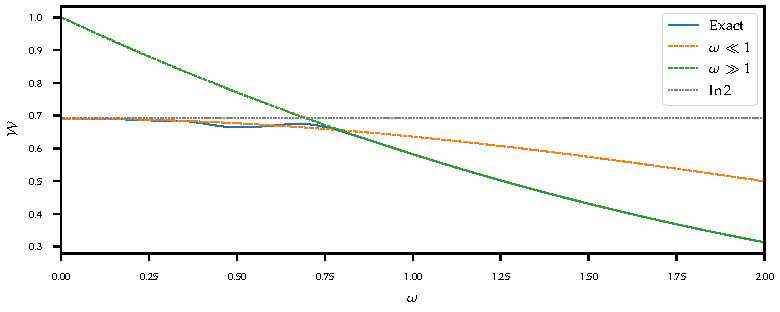
\includegraphics{figs/ergo_calc/ergo_numeric}
  \caption{\label{fig:numeric_n_ho_ergo} Numerical evaluation of
    \cref{eq:many_ho_pass} and the estimates
    \cref{eq:many_ho_ergo_bound,eq:ergo_esti_high_t} for \(N=110\)
    and \(β=1\). Good agreement can be found and the bound
    \(β^{-1}\ln2\) is approximately saturated.}
\end{figure}

In conclusion, we have found an upper bound
\cref{eq:many_ho_ergo_bound} for and a high temperature estimate
\cref{eq:ergo_esti_high_t} of the ergotropy to \(N\) oscillators in a
thermal state and a two level system in a pure state.

\subsection{A bound on the Energy Change of Multiple Baths in the
  Periodic Steady State}
\label{sec:operational_thermo}
As in the single bath case, some statement about the amount of energy
that can be expected to be extracted in a cyclic manner. An argument
based on entropy may be made for the periodic steady state as was
shown in~\cite{Kato2016Dec} and is reproduced here. We will find the
Clausius form of the second law.

We consider the situation given by the Hamiltonian for a system
coupled to multiple baths under periodic driving
\begin{equation}
  \label{eq:katoineqsys}
  H(t) = H_\sys(t) + ∑_i \qty(H_\bath^i + H_\inter^i(t)).
\end{equation}
Here, \(H_\sys(t)\) is the system Hamiltonian, \(H_\bath^i\) is the
Hamiltonian of the \(i\)-th bath and \(H_\inter^i(t)\) is the coupling
to the same. Again, the bath must be treated as finite during the
derivation.

The von Neumann entropy \(S(t)=-\tr[ρ\ln ρ]\) of the global state whose
evolution is generated by \cref{eq:katoineqsys} is
constant. Additionally \(S\) is sub-additive meaning
\begin{equation}
  \label{eq:subadd}
  S(t) \leq -\tr[ρ_\sys(t)\ln ρ_\sys(t)] - ∑_i\tr[ρ_{\bath^i}(t)\ln
  ρ_{\bath^i}(t)] \equiv S_\sys(t) + ∑_iS_{\bath^i}(t),
\end{equation}
where \(ρ_{\sys}(t)=\tr_{\bigotimes_i{\bath^i}}[ρ(t)]\) and
\(ρ_{\bath^i}=\tr_{\sys\bigotimes_{j\neq i}{\bath^j}}[ρ(t)]\) are the
marginal states of system and the \(i\)th bath respectively. Note that
the marginal entropies \(S_{\sys},\,S_{\bath}\) are generally
\emph{not} constant in time.

This implies for \(ΔS_\sys(t)\equiv S_\sys(t) - S_\sys(0)\) and
\(ΔS_{\bath^i}(t)\equiv S_{\bath^i}(t) - S_{\bath^i}(0)\)
\begin{equation}
  \label{eq:deltagreat}
  ΔS_\sys(t) + ∑_i ΔS_{\bath^i}(t) \geq 0.
\end{equation}

The von Neumann entropy of a single bath can be expressed as
\begin{equation}
  \label{eq:bathentro}
  \begin{aligned}
  S_{\bath^i}(t) &=-\tr[ρ_{\bath^i}(t)\ln ρ_{\bath^i}^β] -
                   \qty(\tr[ρ_{\bath^i}\ln ρ_{\bath^i}(t)] -
                   \tr[ρ_{\bath^i}(t)\ln ρ_{\bath^i}^β])\\
                 &= β E_{\bath^i}(t) - βF_{\bath^i} - \qrelent{ρ_{\bath^i}(t)}{ρ_{\bath^i}^β},
  \end{aligned}
\end{equation}
where
\(E_{\bath^i}(t)=\tr[ρ_{\bath^i}(t)H_{\bath^i}]=\tr[ρ(t)(H_{\bath^i}\otimes
\id)]\), \(ρ_{\bath^i}^β=\exp(-β H_{\bath^i})/Z\) and
\(F_{\bath^i}=-\ln(Z_{\bath^i})/β\) is the equilibrium free energy of
the bath at (as yet undetermined) inverse temperature \(β\).
The result \cref{eq:bathentro} implies
\begin{equation}
  \label{eq:bathenergychange}
  ΔS_{\bath^i}(t) = β_i ΔE_{\bath^i}(t) -
  \qrelent{ρ_{\bath^i}(t)}{ρ_{\bath^i}^{β_i}} \leq β_i ΔE_{\bath^i}(t).
\end{equation}
Note that \(β_i\) is now being fixed through
\(\qrelent{ρ_{\bath^i}(0)}{ρ_{\bath^i}^{β_i}}\Leftrightarrow
{ρ_{\bath^i}(0)}={ρ_{\bath^i}^{β_i}}\).

Combining \cref{eq:bathenergychange,{eq:deltagreat}} yields
\begin{equation}
  \label{eq:bathenergyandsystementro}
  ΔS_\sys(t) + ∑_iβ_i ΔE_{\bath^i}(t) \geq 0.
\end{equation}
This inequality only contains quantities that can be expected to be
finite, even in the limit of infinite baths.

As in \cref{sec:ergoonebath} we now demand periodic driving, that is
\(H(t+τ) = H(t)\) for some \(τ\geq 0\). Now we \emph{Assume} that the
system enters a periodic steady state after the time \(n_0τ\) for some
\(n_0\in\NN\) so that \(ρ_\sys((n + n_0)τ)= ρ_\sys(n_0τ)\) for all
\(n\in\NN\). This assumption is linked to the notion of a ``finite
memory'' of the baths. In the same spirit, we \emph{assume} that the
energy change of each bath
\(ΔE_{\bath^i}^\cyc =ΔE_{\bath^i}((n+1)τ)-ΔE_{\bath^i}(nτ) =
E_{\bath^i}((n+1)τ)-E_{\bath^i}(nτ)\) is constant once the system is
in the periodic steady state. This behavior, at least on the system
level, is suggested by the NMQSD equation \cref{{eq:multinmqsd}}.

As the system entropy does not change over a cycle
\(ΔS_\sys^\cyc = ΔS_\sys(τ (n+n_0)) - ΔS_\sys(τ n_0)=S_\sys(τ (n+n_0)) - S_\sys(τ
n_0)=0\) vanishes we have
\begin{equation}
  \label{eq:secondlaw_cyclic}
  ∑_iβ_i ΔE_{\bath^i}^\cyc \geq 0,
\end{equation}
as otherwise the inequality \cref{eq:bathenergyandsystementro} would
be violated in finite time.

If one defines heat as the energy change of the baths as is done
in~\cite{Kato2016Dec} and substantiated, based on a microscopic
definition of entropy, in~\cite{Strasberg2021Aug}\footnote{In this
  work, a full dynamical theory is being derived.},
\cref{eq:secondlaw_cyclic} amounts to the Clausius form of the second
law. This definition of heat is corroborated in~\cite{Esposito2015Dec}
where it is shown\footnote{for fermionic baths} that a definition of heat
involving any nonzero fraction of the interaction energy will lead to
the internal energy (as defined by the first law) not being an exact
differential.

In contrast to~\cite{Strasberg2021Aug}, no interpretation in terms of
thermodynamical quantities is required for \cref{eq:secondlaw_cyclic}
to be useful.  Assume that the interaction Hamiltonian in
\cref{eq:katoineqsys} vanishes periodically, so that system and bath
energy expectation values can be cleanly separated. In the periodic
steady state the system energy does not change during a cycle, so the
whole energy change amounts to the change in bath energy. In a setting
with two baths \cref{eq:secondlaw_cyclic} implies the Carnot bound.

% LocalWords:  ergotropy
